%%%% PGCT submission draft in the IJCAI-27 template (ijcai27.sty, named.bst from the official author kit).
%%%% Intended engine: pdfLaTeX (e.g. Overleaf). The \pdfinfo shim below only matters for XeTeX/Tectonic builds.
\documentclass{article}
\pdfpagewidth=8.5in
\pdfpageheight=11in

\usepackage{ijcai27}

\usepackage{times}
\usepackage{soul}
\usepackage{url}
\usepackage[hidelinks]{hyperref}
\usepackage[utf8]{inputenc}
\usepackage[small]{caption}
\usepackage{graphicx}
\usepackage{amsmath}
\usepackage{amsthm}
\usepackage{booktabs}
\usepackage{algorithm}
\usepackage{algorithmic}
\usepackage[switch]{lineno}
\usepackage{amssymb}
\usepackage{xcolor}
\usepackage{tikz}
% Local XeTeX/Tectonic builds only: metric-compatible Times/Helvetica clones. pdfLaTeX skips this block.
\ifdefined\XeTeXrevision\usepackage{fontspec}
  \setmainfont{texgyretermes}[Extension=.otf,UprightFont=*-regular,BoldFont=*-bold,ItalicFont=*-italic,BoldItalicFont=*-bolditalic]
  \setsansfont{texgyreheros}[Extension=.otf,UprightFont=*-regular,BoldFont=*-bold,ItalicFont=*-italic,BoldItalicFont=*-bolditalic]\fi

% Comment out this line in the camera-ready submission
\linenumbers

\urlstyle{same}

% Shared colours and TikZ styles for the PGCT papers and slides (requires tikz, xcolor).
\usetikzlibrary{arrows.meta,positioning,calc,fit,backgrounds,shapes.geometric}
\definecolor{pgblue}{HTML}{1F4E9A}
\definecolor{pgsky}{HTML}{DCE7F7}
\definecolor{pgorange}{HTML}{C0504D}
\definecolor{pgsand}{HTML}{FBE9DA}
\definecolor{pggreen}{HTML}{2E7D4F}
\definecolor{pgmint}{HTML}{E2F2E8}
\definecolor{pggrey}{HTML}{6B6B6B}
\definecolor{pglight}{HTML}{F4F4F4}
\tikzset{
  pg/.style={font=\sffamily\small},
  stage/.style={draw=pgblue,line width=.8pt,rounded corners=3pt,fill=white,align=center,
                minimum height=1.25cm,text width=2.7cm,inner sep=3pt},
  card/.style={draw=pggrey,rounded corners=2pt,fill=white,align=center,inner sep=2.5pt,font=\sffamily\scriptsize},
  box/.style={draw=pgblue,line width=.8pt,rounded corners=3pt,fill=white,align=center,inner sep=4pt},
  flow/.style={-{Stealth[length=2.4mm]},line width=.9pt,draw=pgblue},
  flowg/.style={-{Stealth[length=2.2mm]},line width=.8pt,draw=pggrey},
  flowo/.style={-{Stealth[length=2.4mm]},line width=.9pt,draw=pgorange},
  band/.style={rounded corners=5pt,inner sep=7pt},
  num/.style={circle,fill=pgblue,text=white,font=\sffamily\bfseries\scriptsize,inner sep=1.2pt,minimum size=4mm},
  lbl/.style={font=\sffamily\scriptsize,text=pggrey,align=center},
}
\newcommand{\stagetitle}[1]{{\bfseries\color{pgblue}#1}}

% Shared verbatim by the English and Korean manuscripts. Numbers follow invocation order.
\newcommand{\ModelEquation}{\begin{equation}\label{eq:model}
 \widehat r_i(q;\psi_i)=\operatorname{MLP}_{\psi_i}
 [u_t,\operatorname{onehot}(a_t),u_{t+1}],\quad u_t=P(o_{i,t}).
\end{equation}}
\newcommand{\RewardLossEquation}{\begin{equation}\label{eq:rloss}
 \mathcal L_i^r=\mathbb E_{(q,r_i)\sim\mathcal B_i^{\rm mix}}
 [(\widehat r_i(q;\psi_i)-r_i)^2].
\end{equation}}
\newcommand{\ProbeEquation}{\begin{equation}\label{eq:probe}
 \mathcal Q_{ij}^{u}=\mathcal E_i^{u}\cup\mathcal E_j^{u}.
\end{equation}}
\newcommand{\DistanceEquation}{\begin{equation}\label{eq:distance}
 D_{ij}^{u}=\frac{\sum_{q\in\mathcal Q_{ij}^{u}}|\widehat r_i^{\,u}(q)-\widehat r_j^{\,u}(q)|}
 {\sum_{q\in\mathcal Q_{ij}^{u}}\big(|\widehat r_i^{\,u}(q)|+|\widehat r_j^{\,u}(q)|\big)}.
\end{equation}}
\newcommand{\ApprovalEquation}{\begin{align}\label{eq:approval}
 \bar D_{ij}&\leftarrow (1-\beta)\bar D_{ij}+\beta D_{ij}^{u},\quad\beta=0.35,\\
 B_{ij}&=\mathbf 1[i\ne j,\ n_{ij}\ge3,\ \bar D_{ij}<0.5,\ m_i^{u}=m_j^{u}=1].\nonumber
\end{align}}
\newcommand{\DonorEquation}{\begin{align}\label{eq:donor}
 C_{ij}^{u}&=\mathbf1[\exists t\text{ in rollout }u:\|p_{i,t}-p_{j,t}\|_\infty\le r_c],\\
 \mathcal G_i^u&=\{j\ne i:C_{ij}^u B_{ij}=1\}.\nonumber
\end{align}}
\newcommand{\MaxEquation}{\begin{align}\label{eq:max}
 b_{i,t}&=\Big[\max_{j\in\mathcal G_i^u}V_j(\tilde h_{i,t}^{\,j})-V_i(h_{i,t})\Big]_+,\\
 f_{i,t}&=V_i(h_{i,t})+w_t b_{i,t}.\nonumber
\end{align}}
\newcommand{\GAEEquation}{\begin{align}\label{eq:gae}
 \delta_{i,t}^{f}&=r_{i,t}+\gamma(1-d_t)f_{i,t+1}+\gamma z_{i,t}^{f}-f_{i,t},\\
 A_{i,t}^{f}&=\delta_{i,t}^{f}+\gamma\lambda_f(1-d_t)A_{i,t+1}^{f}.\nonumber
\end{align}}
\newcommand{\BlendEquation}{\begin{align}\label{eq:blend}
 A_{i,t}^{\rm PGCT}&=A_{i,t}^{\rm self}+\eta\, s_i\, w_t\big(A_{i,t}^{f}-A_{i,t}^{\rm self}\big),\qquad \eta=0.5,\\
 s_i&=\min\!\left(1,\frac{\operatorname{std}_t A_{i,t}^{\rm self}}
 {\max\!\big(\operatorname{std}_t\, w_t(A_{i,t}^{f}-A_{i,t}^{\rm self}),\,10^{-8}\big)}\right).\nonumber
\end{align}}
\newcommand{\PPOEquation}{\begin{align}\label{eq:ppo}
 \rho_{i,t}(\theta_i)&=\pi_{\theta_i}(a_{i,t}\mid h_{i,t})/\pi_{\theta_i^{\rm old}}(a_{i,t}\mid h_{i,t}),\\
 L_i^\pi&=\mathbb E_t[\min\{\rho_{i,t}\widetilde A_{i,t},
 \operatorname{clip}(\rho_{i,t},1-\epsilon,1+\epsilon)\widetilde A_{i,t}\}],\nonumber\\
 R_{i,t}^{\rm self}&=A_{i,t}^{\rm self}+V_i^{\rm old}(h_{i,t}).\nonumber
\end{align}}
\newcommand{\BoundEquation}{\begin{equation}\label{eq:bound}
 \|\Delta A\|_\infty\le\left(1+\frac{\gamma(1-\lambda)}{1-\gamma\lambda}\right)\|\Delta f\|_\infty.
\end{equation}}


% XeTeX has no \pdfinfo primitive; pdfLaTeX ignores this line.
\ifdefined\pdfinfo\else\def\pdfinfo#1{\special{pdf:docinfo<<#1>>}}\fi

% PDF Info Is REQUIRED.
\pdfinfo{
/TemplateVersion (IJCAI.2027.0)
}

\title{Probe-Gated Critic Transfer: Latent Team Discovery\\from Individual Reward Responses}

\author{HwanRyul Lee}

\begin{document}

\maketitle

\begin{abstract}
Agents that share a workspace need not share a goal. We study online latent team discovery in fully decentralized multi-team reinforcement learning, where each agent observes only its own observations and individual reward, team labels are never given, and agents communicate only on physical contact. We propose Probe-Gated Critic Transfer (PGCT). Each agent learns a predictor of its own reward. When two agents meet, both predictors answer a common set of public reward-event probes, and a normalized response distance, smoothed over rounds, approves persistent agreement; agents without enough reward experience abstain. To test whether the discovered relation is useful, an approved teammate's Critic evaluates the receiver's own history, and its positive uplift enters a masked, scale-limited Max-GAE advantage for the Actor only, while every Critic keeps learning its own return. In a six-agent, two-team warehouse task, discovery separates teammates from about 0.25M steps (response distance 0.25 versus 0.99) and directs 93.7\% of approved peer access to true teammates over 5M steps. Learning comparisons of the integrated method are in progress.
\end{abstract}

\section{Introduction}
Cooperation in multi-agent reinforcement learning (MARL) usually assumes that the cooperating group is known. A shared team reward, a centralized Critic, or parameter sharing all presuppose which agents belong together \cite{mappo,seps}. In many deployments this assumption is not available. Several teams of robots may work in the same warehouse, each team serving its own request queue and delivering to its own goal. An agent sees its neighbors, but proximity does not reveal whether a neighbor pursues the same task. If the agent shares value information indiscriminately, estimates learned for different goals are mixed. If it never shares, it cannot benefit from a teammate that has already learned the task.

We therefore ask two questions. \textbf{Q1 (discovery):} can an agent identify its latent teammates online, using only its own experience and local communication? \textbf{Q2 (use):} once teammates are identified, does their value information help the agent learn? Q1 is the main subject of this paper; Q2 serves to test whether the discovered relation is useful for learning.

A natural signal for Q1 is policy similarity. However, policies of agents with the same task can differ while they learn, and agents with different tasks can behave alike when both act almost randomly. We instead use the quantity that defines a task: the reward. Agents of the same team receive reward under the same rule, so the same event should be rewarding for both. Agents of different teams are rewarded for different events. Each agent can learn this rule from its own reward without sharing any reward value. Two agents then compare what their reward predictors say about a common set of public events. This comparison raises three difficulties. Reward events are sparse. Observations contain task-private channels that must not be exchanged. And an agent without reward experience has no reward rule to compare.

\paragraph{Contributions.} (i) We formulate online latent team discovery in fully decentralized multi-team MARL with individual rewards, no team labels and contact-limited communication. (ii) We propose a reward-response probe test for discovery: each agent learns a predictor of its own reward from public transitions; agents that meet compare predictions on common reward-event probes with a scale-free distance; persistent agreement approves the pair, agents without enough own reward evidence abstain, and only information that existed at the time of contact enters the comparison. (iii) We use the discovered relation through selective peer-Critic access: an approved teammate's Critic evaluates the receiver's own history, and its positive uplift shapes the Actor advantage through a masked, scale-limited Max-GAE term, while each Critic keeps its own-return target and the method reduces exactly to independent PPO when no teammate is approved. (iv) In a warehouse task, we report discovery during training, an offline replay of the discovery rule, online discovery by the complete method, and a counterfactual check of why the team relation matters for peer values.

\section{Related Work}
\paragraph{Independent and shared learning.}
Independent learners optimize their own objective and remain strong baselines in cooperative MARL \cite{tan,ippo,benchmark}. PPO and generalized advantage estimation (GAE) are standard components of such learners \cite{ppo,gae,mappo}. Shared Experience Actor-Critic shares experience among cooperating agents \cite{seac}. Selective parameter sharing groups agents before sharing parameters \cite{seps}. Fully decentralized actor-critic methods let networked agents reach consensus on a common Critic \cite{fdmarl}. These methods assume that the group with a common objective is given, or that all agents share one objective. PGCT instead infers the group from individual rewards and keeps separate Actors and Critics.

\paragraph{Modelling other agents.}
Agent modelling infers properties of other agents, such as goals, types or policies \cite{modelling}. Ad hoc teamwork asks an agent to cooperate with unknown teammates without prior coordination \cite{adhoc}. Our inferred object is narrower: whether another agent is rewarded by the same rule. The inference uses the agent's own reward predictor and a peer's predictions on public events. It requires no model of the peer's policy.

\paragraph{Combining several value functions.}
Generalized policy improvement combines value functions of several policies through a maximum \cite{gpi}. MAMBA uses the statewise maximum of several oracle values inside a GAE-style estimator and gives improvement guarantees when these oracle values are estimated in the learner's state distribution \cite{mamba}. Our Max-GAE term follows this aggregation idea. Its premises are not met, however. A peer Critic is trained on the peer's own histories and is evaluated on the receiver's history; it is not an oracle value re-estimated by rollouts. We therefore claim no performance guarantee and treat the peer value as an auxiliary Actor signal whose effect must be measured.

\section{Problem Setting}
Consider $N$ agents in a partially observable environment. Agent $i$ receives an observation $o_{i,t}$, takes an action $a_{i,t}$ and receives its own scalar reward $r_{i,t}$. Each agent has a hidden team label $z_i$, and agents of one team are rewarded by the same rule. Two agents are \emph{latent teammates} if $z_i=z_j$. Labels are used only for evaluation and for oracle baselines.

\paragraph{Information model.}
Each agent keeps its own recurrent Actor and Critic. Agents $i$ and $j$ can communicate during rollout $u$ only if they come within Chebyshev distance $r_c$ at some step:
\DonorEquation
We take the communication radius equal to the observation radius ($r_c=5$ in our task), so an agent can talk to the agents it can see; the radius of the reported runs is stated in Section~\ref{sec:setup}. On contact, agents may exchange public event views, their predicted rewards on those views and Critic weights. They never exchange reward values, team labels, Actor weights or private trajectories. A public projection $P$ removes task-private observation channels (requested shelves and the agent's own goal) and absolute coordinates. In the implementation, $P(o)$ keeps six ego features and eleven physical grid channels within radius two, a 281-dimensional view. Actor and Critic use the full semantic observation with the two coordinate entries set to zero.

\paragraph{Goal.}
Each agent should estimate the relation $\mathbf 1[z_i=z_j]$ for agents it meets, abstain when it lacks evidence, and use the estimate to improve its own learning without changing its own reward or its Critic's target.

\section{Probe-Gated Critic Transfer}
\begin{figure*}[t]
\centering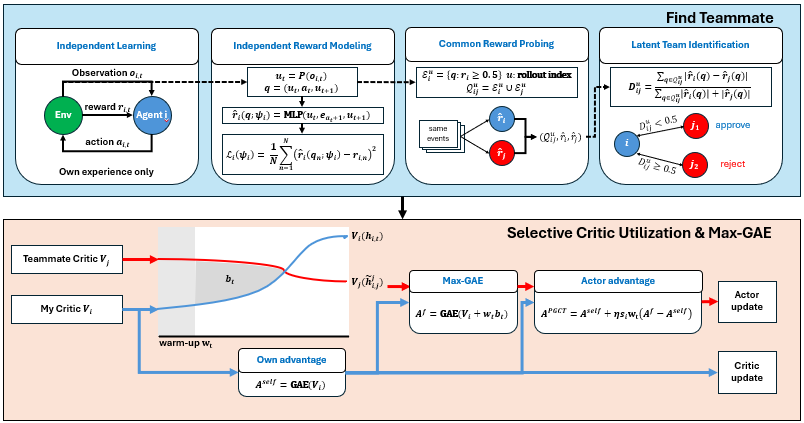
\includegraphics[width=.97\textwidth]{figures/fig_overall.png}
\caption{Overall PGCT procedure for agent $i$. Top: the agent learns from its own experience, fits a reward predictor on public transitions, compares its predictions with those of a peer it met on common reward-event probes, and approves the peer when the response distance is small (simplified; the full rule is Eq.~\ref{eq:approval}). Bottom: the Critic of an approved teammate raises the value input of GAE by the positive uplift $b_t$; the result changes only the Actor update, and the Critic keeps learning its own return. All computation is local; peers exchange public event views, predicted responses and Critic weights only on contact.}\label{fig:architecture}
\end{figure*}

Figure~\ref{fig:architecture} shows the two parts of PGCT: team discovery (top) and selective Critic use (bottom). Algorithm~\ref{alg:pgct} lists one update; steps 1--4 answer Q1 and steps 5--7 answer Q2.

\subsection{Individual Reward Prediction}
Each agent fits a multilayer perceptron to its own reward on public transitions $q=(u_t,a_t,u_{t+1})$:
\ModelEquation
The input has $281+5+281=567$ dimensions, and the hidden layers have 128 and 64 ReLU units. Each agent stores its last 20{,}000 transitions and, separately, its last 512 reward events. An event is a transition with own reward $r_i\ge0.5$; in our task these are deliveries and shelf returns. Events make up less than 0.5\% of transitions, so a quarter of every training batch is drawn from the event buffer. The loss is
\RewardLossEquation
Every five PPO updates, the predictor takes 50 Adam steps (batch 256, learning rate $10^{-3}$). Because public views hide task-private information, the same public transition can be rewarding or not. The regression then learns the conditional mean of the reward, which is the quantity we compare.

\subsection{Reward Probes}
When $i$ and $j$ have met during rollout $u$, they build a common probe set
\ProbeEquation
Here $\mathcal E_i^u$ is the public view of the 32 most recent own events of agent $i$ recorded before rollout $u$ starts. Probes are concatenated with repetitions. Reward values are never part of a probe. The two event sets already contain the question that separates teams when both agents have rewarded events: a delivery at one goal is rewarding for one team and not for the other. When the map has a known left--right symmetry, the probe set can optionally be augmented with mirrored copies $M(\mathcal E_i^u\cup\mathcal E_j^u)$, where $M$ mirrors views and turning actions; this adds an assumption about the map and is not part of the core method. Our runs use this augmentation (Section~\ref{sec:setup}).

\paragraph{Causal snapshot.}
Comparisons happen at the end of a rollout, but a pair may have met early in it. To use only information that existed at contact time, each agent freezes its event probes, its maturity flag and its predictor version at the start of rollout $u$. Predictors are refitted only after a rollout, so the frozen version is exactly the predictor used during the rollout. The comparison for rollout $u$ uses this frozen state and is performed before the predictors are refitted.

\begin{figure}[t]
\centering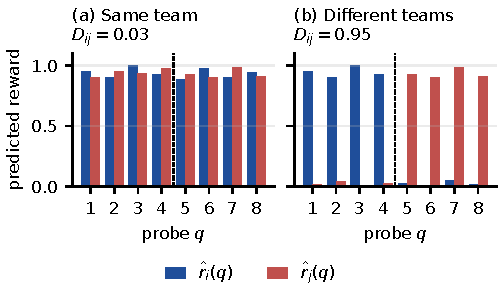
\includegraphics[width=\columnwidth]{figures/fig_discovery.pdf}
\caption{Reward-based team discovery for a pair of agents that met (illustration, not data). Both reward predictors answer the common probes; probes 1--4 are reward events of agent $i$ and probes 5--8 of agent $j$. (a) Teammates predict reward on every probe, so the response distance is near 0. (b) Agents of different teams predict reward only on their own events, so the distance is near 1. Agents without enough own reward events abstain.}\label{fig:discovery}
\end{figure}

\subsection{Response Distance and Team Discovery}
Both predictors evaluate the same probes (Figure~\ref{fig:discovery}). Their discrepancy is
\DistanceEquation
Probes on which both predictors answer zero add nothing to the numerator or the denominator. Many uninformative probes therefore do not dilute the distance. If the denominator is below $10^{-8}$ the comparison abstains. An agent is \emph{mature} ($m_i^u=1$) if it has observed at least 20 own events, its predictor has been fitted, and its mean prediction on its own recent events is at least 0.3. Pairs are compared every five updates and only if both agents are mature. The distance is smoothed across comparison rounds and the pair is approved by
\ApprovalEquation
Here $n_{ij}$ counts rounds in which both predictors were refitted on new experience. The approval is symmetric and persists when the agents lose contact; a stale approval is used only if the pair meets again. The threshold 0.5 means that most of the response mass is shared; it is fixed in advance and not tuned on our runs. No team label enters this decision.

\subsection{Selective Peer Critic Access}
The donor set of agent $i$ for rollout $u$ is
\begin{equation}\label{eq:donorset}
\mathcal G_i^u=\{j\ne i: C_{ij}^u=1,\ B_{ij}=1\}.
\end{equation}
Donor Critic weights are those used during rollout $u$ and are received on contact; they are frozen during the update. Agent $i$ replays its own observation sequence through each donor Critic and obtains a donor-specific recurrent state $\tilde h^{\,j}_{i,t}$. The donor's hidden state is never sent. The replay starts from a zero state at the rollout boundary and resets at episode ends. Until eight observations have passed or the first reset occurs, the replayed value is not yet reliable, and a mask $w_t=0$ removes it.

\begin{algorithm}[tb]
\caption{One PGCT update of agent $i$}
\label{alg:pgct}
\begin{algorithmic}[1]
\STATE At rollout start, freeze event probes, maturity flag and predictor version.
\STATE Collect the rollout; store own public transitions and own events; record contacts $C^u_{ij}$.
\IF{the update index is a multiple of five}
\STATE Compare contacted mature pairs on frozen probes; update $\bar D_{ij}$ and $n_{ij}$ (Eqs.~\ref{eq:distance}--\ref{eq:approval}).
\STATE Refit the reward predictor on own experience (Eq.~\ref{eq:rloss}).
\ENDIF
\STATE Donors: approved peers met in this rollout (Eq.~\ref{eq:donorset}).
\STATE Replay own history through donor Critics; compute $b$, $f$ and $A^{\rm PGCT}$ (Eqs.~\ref{eq:max}--\ref{eq:blend}).
\STATE Update the Actor by PPO with $A^{\rm PGCT}$ and the Critic toward its own return (Eq.~\ref{eq:ppo}).
\end{algorithmic}
\end{algorithm}

\subsection{Max-GAE Advantage Estimation}
For a nonempty donor set, the positive uplift and the combined value are
\MaxEquation
The GAE recursion uses the trainer's termination and time-limit handling:
\GAEEquation
where $d_t$ marks episode ends and $z^f_{i,t}$ is the value of a captured time-limit observation (zero otherwise). The self advantage $A^{\rm self}$ uses the same recursion with $V_i$ in place of $f$. With $\gamma=0.99$ and $\lambda_f=\lambda=0.95$, the Actor advantage is
\BlendEquation
The lower half of Figure~\ref{fig:architecture} shows the computation. Two details matter. First, the mask $w_t$ multiplies the advantage difference $A^f-A^{\rm self}$, not only $b$. Masking only $b$ would let future uplift leak into the cold-start steps through the GAE recursion. Second, the factor $s_i\le1$ shrinks a large auxiliary term to the scale of the agent's own advantage but never inflates a small one. In our task the raw difference was 2.6--12 times $\operatorname{std}A^{\rm self}$ for lagging agents. Without $s_i$, PPO's advantage normalization would make the result almost independent of $\eta$.

\subsection{Actor and Critic Updates}
After per-agent normalization, write the Actor advantage as $\widetilde A_{i,t}$. PPO uses
\PPOEquation
The Actor maximizes the clipped objective plus an entropy bonus. The Critic minimizes the trainer's clipped value loss toward its own return $R^{\rm self}$; there is no peer distillation loss. Actor and Critic have separate encoders and recurrent layers. They share one gradient-norm clip, so a different Actor advantage can change the effective Critic step size but not its target.

\section{Properties}
\paragraph{Bounded, scale-free distance.} By the triangle inequality, $D_{ij}^u\in[0,1]$ whenever its denominator is positive. The distance does not depend on the reward scale shared by both predictors.

\paragraph{A necessary condition for discovery.} If two reward rules induce the same predictor responses on every public probe available to the agents, no rule that sees only these responses can tell them apart. Discovery therefore requires task-discriminating public reward events. An agent that has never received a qualifying reward has no response to compare, and PGCT abstains for it by design.

\paragraph{Reduction to independent PPO.} If $\mathcal G_i^u=\emptyset$ or $b_{i,t}=0$ for all $t$, then $A^{f}=A^{\rm self}$ and therefore $A^{\rm PGCT}=A^{\rm self}$. Because $s_i\le1$, the change $|A^{\rm PGCT}-A^{\rm self}|$ goes to zero as the uplift does. For a fixed donor set, unmasked steps and fixed $s_i$, GAE is linear in its value input, and the Actor advantage equals GAE computed with $V_i+\eta s_i w_t b_i$.

\paragraph{Sensitivity to value errors.} For bounded value perturbations $\Delta f$ on continuing trajectories,
\BoundEquation
This bounds how a peer-value error can move the advantage. It is not a performance guarantee: the peer value is extrapolated to another agent's histories, other agents keep learning, and contacts change between rollouts.

\section{Experiments}
\begin{figure*}[t]\centering
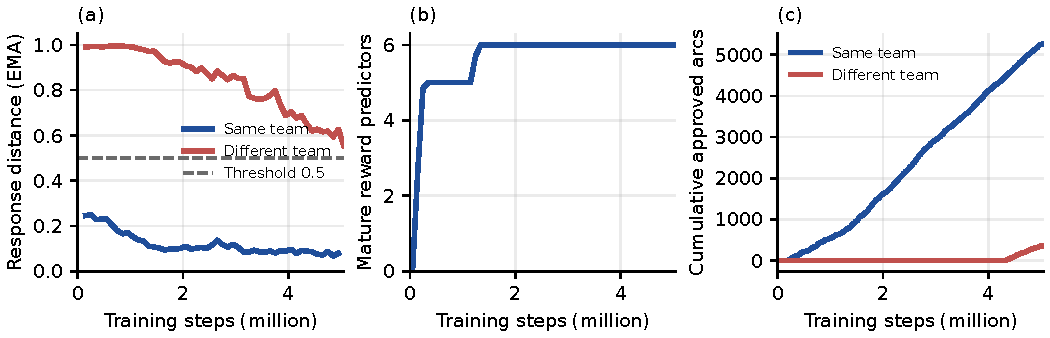
\includegraphics[width=.98\textwidth]{figures/discovery_log.pdf}
\caption{Discovery in the warehouse task (corner goals, individual rewards, seed 1, 5M steps). (a) Mean response-distance EMA of compared pairs, 100k-step bins; the dashed line is the approval threshold. (b) Number of agents with a mature reward predictor. (c) Cumulative directed peer-access arcs by true relation.}\label{fig:gate-data}
\end{figure*}

\subsection{Setup}\label{sec:setup}
\paragraph{Environment.} We use a multi-team variant of the robotic warehouse \cite{benchmark}: an $11\times10$ grid with six agents in two teams of three. The team goals are at the two bottom corners, $(0,10)$ and $(9,10)$. Each team has three requested shelves. Observations are semantic grids with sensor radius five. Every agent receives its own reward: 1 for a delivery, 1 for a shelf return, 0.15 for picking up a requested shelf, small progress terms (0.02, 0.005, 0.002) and small penalties (0.002--0.05) for unproductive actions. No team reward is used. Table~\ref{tab:settings} lists the learning settings. The reported runs differ from the default method in two settings: they use a contact radius $r_c=3$, smaller than the observation radius, and they augment probes with mirrored copies. A contact within radius 3 is also a contact within radius 5, so the default only adds contacts; without mirrors, an offline replay gave the same decisions (Section~\ref{sec:discovery}). Runs with $r_c=5$ and without mirrors are pending.

\begin{table}[t]\centering\small
\begin{tabular}{lr}\toprule
Setting & Value\\\midrule
Rollout / recurrent sequence & 1024 / 64 steps\\
PPO epochs / minibatches & 4 / 8\\
Learning rate / entropy & $2\times10^{-4}$ / 0.05\\
PPO clip / value clip & 0.2 / 0.2\\
Discount / GAE parameter & 0.99 / 0.95\\
Encoder / GRU width & 128 / 128\\
Reward fit: interval / steps & 5 updates / 50\\
Event threshold / maturity & $r\ge0.5$ / 20 events\\
EMA $\beta$ / threshold / rounds & 0.35 / 0.5 / 3\\
Contact radius $r_c$ (Chebyshev), runs & 3\\
Mirrored probes, runs & yes\\
Max-GAE $\eta$ / scale & 0.5 / shrink\\\bottomrule
\end{tabular}
\caption{Environment interaction and PGCT settings.}\label{tab:settings}
\end{table}

\paragraph{Branch runs.} To run the complete method online, we branch from a common independent-PPO checkpoint at 1.024M steps (seed 1) and train for 0.5M further steps with seeds 1, 3 and 5, which keep the checkpoint's goal layout. At this checkpoint three agents ($a_0,a_1,a_4$) deliver little or nothing. As a control, the same branches are run with true teammates as donors, restricted to agents with mature predictors; these runs log the same discovery statistics. Branch seeds continue one training run and are not independent training seeds.

\subsection{Team Discovery}\label{sec:discovery}
Figure~\ref{fig:gate-data} shows a 5M-step run (seed 1) in which the discovery rule of PGCT was active. Same-team and different-team pairs separate as soon as agents mature. In the 0.1--0.25M bin, the mean response distance is 0.25 for teammates and 0.99 for others, and five of six agents are mature by 0.25M. The same-team distance keeps falling (0.08 after 4M). The different-team distance stays near 0.99 until about 1M and then slowly declines. Over the run, 5{,}252 directed peer-access arcs went to true teammates and 352 to agents of the other team, a same-team share of 93.7\%. The first different-team approval appears at 4.28M steps, so all access before that point was correct. This share is weighted by access frequency and is not a pair-level accuracy. The run used update-end positions as contacts and an earlier peer-usage rule, so it evaluates the discovery component only.

As an offline check, we replayed a subsample of the experience of a completed independent-PPO run (0.26--5M steps, about 1/180 of its transitions) through the same rule, assuming every pair is in contact at every round. Of the 15 pairs, the 10 that reached a decision were all classified correctly: four same-team approvals and no different-team approval (same-team distances 0.14--0.18, different-team 0.58--0.70). The other five pairs all involved the one agent that never learned to deliver, and they abstained. Removing the mirrored probes from this replay left every decision unchanged.

The branch runs (Section~\ref{sec:setup}) execute the complete method online, with rollout-start snapshots and the contact rule. In the three PGCT branches (seeds 1, 3 and 5; seed 5 up to 0.46M of its 0.5M steps), no different-team pair was ever approved, and all donor arcs used by Max-GAE went to true teammates (1{,}920, 1{,}350 and 1{,}258). The first approval came 20k--26k steps after branching. Four agents became mature in each run: all three agents of one team and one agent of the other. PGCT approved all six directed arcs inside the first team and none of the six arcs between the lone mature agent and that team, so it found 6 of the 12 same-team arcs and abstained on the rest. The three control runs also log no different-team approval. These branches cover 1.02--1.52M training steps, before the late decline of the different-team distance seen in the 5M run.

\subsection{Why the Team Relation Matters for Peer Values}
Is a teammate's Critic useful only for teammates? We ran a counterfactual check on saved checkpoints of independent PPO. From the same environment state, we let a lagging agent act either with its own policy or with a peer's policy, while all other agents kept their own policies, and compared the lagging agent's own return over 100 steps (common random numbers, 8 repetitions). Across four checkpoint datasets (two time points of one run and two runs of an earlier configuration with visible coordinates), when a same-team peer Critic predicted an uplift above 0.2 for the lagging agent, the peer's policy actually increased the agent's return in 67--100\% of cases, with mean gains of 0.28--0.58. Different-team uplifts of similar size corresponded to mean gains of only $-0.01$ to $0.14$. For leading agents, different-team Critics often predicted uplifts that came with significant losses. The predicted uplift also overestimated the real gain by up to a factor of 1.6. These observations motivate both the discovery step and the conservative scaling of the uplift.

\section{Limitations}
Discovery depends on reward experience. Agents that never receive a qualifying reward cannot be matched, and they may be exactly the agents that need help most: in the PGCT branch runs, two of the three lagging agents ($a_0,a_4$) never became mature, so PGCT abstained for them. Late in the 5M run, the different-team distance declines and a few cross-team approvals appear; the cause is not yet analyzed. A peer Critic estimates returns under the peer's own policy, so its value on another agent's history can be biased, and the maximum can amplify this bias. Whether selective Critic use speeds up learning is not yet shown, and the current evidence comes from one environment family and few seeds.

\section{Conclusion}
PGCT discovers latent teammates online from individual reward responses. Each agent predicts its own reward, compares predictions on public reward-event probes with peers it meets, and approves only persistent agreement backed by enough own experience. The discovered relation is used conservatively: approved teammates' Critics shape the Actor advantage through a masked, scale-limited Max-GAE term, and each Critic keeps its own return. In a two-team warehouse, discovery separates teammates early and directs most peer access to true teammates, and in branch runs of the complete method it approved no different-team pair. Whether this access speeds up learning is still being tested.

%% The file named.bst is a bibliography style file for BibTeX 0.99c
\bibliographystyle{named}
\bibliography{references}

\end{document}
